\newpage
{\bfseries МРНТИ 20.23.25}
\hfill {\bfseries \href{https://doi.org/10.58805/kazutb.v.2.23-488}{https://doi.org/10.58805/kazutb.v.2.23-488}}

\sectionwithauthors{М.Мұсайф, А.Ж. Кинтонова, А.Е. Назырова, С.А. Алтынбек, М. Калдарова}{ИНТЕГРАЦИЯ УНИМОДАЛЬНЫХ И МУЛЬТИМОДАЛЬНЫХ БИОМЕТРИЧЕСКИХ СИСТЕМ
ДЛЯ ПОВЫШЕНИЯ ТОЧНОСТИ ИДЕНТИФИКАЦИИ ЛИЧНОСТИ: РАЗРАБОТКА И ОЦЕНКА
МЕТОДА PCA-ДАУГМАНА}

\begin{center}
{\bfseries \textsuperscript{1}М.Мұсайф, \textsuperscript{1}А.Ж. Кинтонова, \textsuperscript{2}А.Е. Назырова, \textsuperscript{3}С.А. Алтынбек , \textsuperscript{2}М. Калдарова}

\textsuperscript{1}Евразийский национальный университет имени Л. Н.
Гумилёва, Астана, Казахстан,

\textsuperscript{2}Международный университет Астана, Астана, Казахстан,

\textsuperscript{3}Казахский университет технологии и бизнеса имени
К.Кулажанова,

e-mail: kzldkz@gmail.com.
\end{center}

В данной статье рассматривается применение унимодальных и
мультимодальных биометрических систем для идентификации личности, с
особым вниманием к аспектам повышения точности распознавания.
Унимодальные системы, которые используют один тип биометрического
признака, такие как радужная оболочка глаза или лицо, широко применяются
в областях, требующих высоких мер безопасности и контроля посещаемости.
Несмотря на их популярность, такие системы сталкиваются с рядом проблем,
включая шум в данных и внутриклассовые различия, что ограничивает их
эффективность.

В работе детально анализируются различные методы и алгоритмы,
используемые в унимодальных системах, включая анализ главных компонентов
(PCA) для распознавания лиц и алгоритм Даугмана для идентификации по
радужной оболочке. Рассматриваются их преимущества и ограничения на
основе последних исследований.

Особое внимание уделяется разработке мультимодальной биометрической
системы, которая объединяет несколько биометрических признаков для
улучшения точности идентификации. В статье предложен новый
комбинированный метод PCA-Даугмана, интегрирующий методы распознавания
лиц и радужной оболочки. Этот подход показывает значительные улучшения в
производительности по сравнению с унимодальными системами, что
подтверждается тестированием на наборах данных ORL, YALE, Real face и
CASIA.

Исследование показывает, что мультимодальная биометрическая система
может эффективно преодолеть ограничения унимодальных систем, предлагая
более высокий уровень безопасности и надежности в идентификации
личности.

{\bfseries Ключевые слова:} биометрию, мультимодальные системы,
распознавание лица, алгоритм Даугмана и анализ главных компонент (PCA),
которые описывают основные технологии и методы, применяемые для
повышения эффективности систем идентификации личности.

\begin{center}
{\large\bfseries ЖЕКЕ СӘЙКЕСТЕНДІРУ ДӘЛДІГІН ЖАҚСАРТУ ҮШІН УНИМОДАЛЬДІ ЖӘНЕ
МУЛЬТИМОДАЛЬДЫ БИОМЕТРИЯЛЫҚ ЖҮЙЕЛЕРДІ БІРІКТІРУ: PCA-DAUGMAN ӘДІСІН
ӘЗІРЛЕУ ЖӘНЕ БАҒАЛАУ}

{\bfseries \textsuperscript{1}М.Мұсайф,\textsuperscript{1}А.Ж.Кинтонова,
\textsuperscript{2}А.Е.Назырова, \textsuperscript{3}С.А.Алтынбек,
\textsuperscript{2}М.Қалдарова}

\textsuperscript{1}Л. Н. Гумилев атындағы Еуразия Ұлттық Университеті,
Астана, Қазақстан,

\textsuperscript{2}Астана Халықаралық Университеті, Астана, Қазақстан,

\textsuperscript{3}Қ. Құлажанов атындағы Қазақ технология және бизнес
университеті, Астана, Қазақстан,

e-mail: kzldkz@gmail.com
\end{center}

Бұл мақалада тану дәлдігін жақсартуға ерекше назар аудара отырып, жеке
сәйкестендіру үшін бірмодальды және мультимодальды биометриялық
жүйелердің қолданылуы қарастырылады. Ирис немесе бет сияқты биометриялық
ерекшеліктердің бір түрін қолданатын бірмодальды жүйелер жоғары
қауіпсіздік шаралары мен сабаққа қатысуды бақылауды қажет ететін
жерлерде кеңінен қолданылады. Танымалдылығына қарамастан, бұл жүйелер
бірнеше қиындықтарға тап болады, соның ішінде деректер шуы және олардың
тиімділігін шектейтін сынып ішіндегі вариациялар.

Мақалада бірмодальды жүйелерде қолданылатын әртүрлі әдістер мен
алгоритмдердің егжей-тегжейлі талдауы, соның ішінде бетті тану Үшін
Негізгі Компоненттерді Талдау (PCA) және иристі анықтау үшін Даугман
алгоритмі берілген. Олардың артықшылықтары мен шектеулері соңғы
зерттеулер негізінде талқыланады.

Сәйкестендіру дәлдігін арттыру үшін бірнеше биометриялық ерекшеліктерді
біріктіретін мультимодальды биометриялық жүйені дамытуға ерекше көңіл
бөлінеді. Мақалада бет пен иристі тану әдістерін біріктіретін ЖАҢА
біріктірілген PCA-Daugman әдісі ұсынылған. Бұл тәсіл бірмодальды
жүйелермен салыстырғанда өнімділіктің айтарлықтай жақсарғанын көрсетеді,
Бұл ORL, YALE, Real face және CASIA деректер жиынтығында тестілеу арқылы
расталады.

Зерттеу көрсеткендей, мультимодальды биометриялық жүйе жеке
сәйкестендіруде қауіпсіздік пен сенімділіктің жоғары деңгейін қамтамасыз
ете отырып, бірмодальды жүйелердің шектеулерін тиімді түрде жеңе алады.

{\bfseries Кілттік сөздер:} биометрия, мультимодальды жүйелер, тұлғаны
тану, Даугман алгоритмі, Жеке Сәйкестендіру жүйелерінің тиімділігін
арттыру үшін қолданылатын негізгі технологиялар мен әдістерді
сипаттайтын Негізгі Компоненттерді Талдау (PCA).

\begin{center}
{\large\bfseries INTEGRATION OF UNIMODAL AND MULTIMODAL BIOMETRIC SYSTEMS TO
IMPROVE THE ACCURACY OF PERSONAL IDENTIFICATION: DEVELOPMENT AND
EVALUATION OF THE PCA-DAUGMAN METHOD}

{\bfseries \textsuperscript{1}M.Mussaif, \textsuperscript{1}A.Kintonova,
\textsuperscript{2}A.Nazyrova, \textsuperscript{3}S.Altynbek,
\textsuperscript{2}M.Kaldarova}

\textsuperscript{1}L. N. Gumilev Eurasian National University, Astana,
Kazakhstan,

\textsuperscript{2}Astana International University, Astana, Kazakhstan,

\textsuperscript{3}K.Kulazhanov Kazakh University of Technology and
Business, Kazakhstan,

e-mail: kzldkz@gmail.com
\end{center}

This article examines the application of unimodal and multimodal
biometric systems for personal identification, with a particular focus
on improving recognition accuracy. Unimodal systems, which use a single
type of biometric feature, such as the iris or face, are widely used in
areas requiring high security measures and attendance control. Despite
their popularity, these systems face several challenges, including data
noise and intraclass variations, which limit their effectiveness.

The paper provides a detailed analysis of various methods and algorithms
used in unimodal systems, including Principal Component Analysis (PCA)
for face recognition and the Daugman algorithm for iris identification.
Their advantages and limitations are discussed based on recent research.

Special attention is given to the development of a multimodal biometric
system that combines multiple biometric features to enhance
identification accuracy. The article proposes a new combined PCA-Daugman
method, integrating face and iris recognition techniques. This approach
shows significant improvements in performance compared to unimodal
systems, as confirmed by testing on ORL, YALE, Real face, and CASIA
datasets.

The study demonstrates that a multimodal biometric system can
effectively overcome the limitations of unimodal systems, offering a
higher level of security and reliability in personal identification.

{\bfseries Keywords:} biometrics, multimodal systems, face recognition,
Daugman algorithm, Principal Component Analysis (PCA), which describe
the main technologies and methods used to enhance the effectiveness of
personal identification systems.

\begin{multicols}{2}
{\bfseries Введение.} Унимодальная биометрическая система определяется как
система, использующая один тип биометрического признака для
идентификации личности, такой как лицо, радужная оболочка или отпечатки
пальцев. Распознавание лиц, в качестве примера такой системы, активно
используется в областях, связанных с безопасностью и контролем
посещаемости {[}1{]}. В литературе представлены различные методы
распознавания лиц, включая анализ главных компонентов (PCA), дискретное
косинусное преобразование, сохраняющие локализацию проекции, линейный
дискриминантный анализ, вейвлеты Габора, независимый компонентный
анализ, нейронные сети, скрытые марковские модели и нечеткие нейронные
сети {[}2{]}. Среди них, анализ главных компонентов (PCA) выделяется как
один из наиболее популярных алгоритмов для распознавания лиц {[}3, 4{]}.

Распознавание радужной оболочки глаза также является примером
унимодальной биометрической системы, которая использует уникальные
характеристики радужной оболочки для идентификации личности. В этой
области применяются различные алгоритмы, включая подход Даугмана, подход
Уайлдса, подход Ли Ма, подход Тиссе, локальные бинарные паттерны (LBP) в
дополнение к методам LVQ и Масека {[}5, 6{]}. Алгоритм Даугмана особенно
выделяется благодаря своей эффективности и популярности.

Однако унимодальные системы сталкиваются с рядом проблем, таких как шум
в данных, ограниченная универсальность и внутриклассовые различия, что
часто приводит к недостаточному уровню производительности. В ответ на
эти ограничения, мультимодальные биометрические системы интегрируют
несколько биометрических признаков, повышая тем самым точность
идентификации {[}7{]}.

В рамках данной работы, были объединены методы распознавания лица и
радужной оболочки глаза для улучшения точности идентификации через
мультимодальную биометрическую систему. Для распознавания лиц
использовался алгоритм PCA на основе наборов данных ORL, YALE и Real
face, в то время как для распознавания радужной оболочки использовался
алгоритм Даугмана с использованием набора данных CASIA. Это позволило
предложить эффективный мультимодальный биометрический метод, названный
комбинированным методом PCA-Даугмана {[}8{]}.

{\bfseries Литературный обзор.} Многочисленные исследования в области
распознавания по радужной оболочке глаза и лицу подчеркивают важность
биометрических данных для идентификации личности. Методы, такие как
анализ главных компонентов (PCA) и метод Даугмана, находят широкое
применение в этой сфере. В одном из исследований был разработан метод,
объединяющий данные радужки и лица для повышения точности распознавания,
с использованием модифицированного PUMP для анализа совокупных
характеристик {[}7{]}. Другое исследование предложило мультимодальную
систему, интегрирующую данные лица, года рождения и радужной оболочки,
дополненную функцией распознавания ушей {[}8{]}. Также была создана
бимодальная система, совмещающая характеристики лица и радужной
оболочки, применяя DCT и PCA-преобразование для улучшения точности
сегментации методом Snake {[}9{]}.

Были обсуждены мультимодальные биометрические системы, объединяющие
отпечатки пальцев, лицо и радужную оболочку, для повышения точности
распознавания и качества изображений, что способствует эффективному
биометрическому анализу {[}10{]}. Исследовалась стратегия гибридного
слияния, объединяющая черты лица и радужной оболочки на уровне принятия
решений, используя данные из наборов ORL face и CASIA iris {[}11{]}.
Применение комбинации биометрических признаков лица и радужной оболочки
с использованием алгоритмов Виолы Джонс и кругового преобразования Хафа
для сегментации, а также MPCA и 2D-фильтра Габора для извлечения
признаков также было исследовано {[}12{]}.

Различные архитектуры CNN, включая AlexNet, VGGNet и ResNet,
демонстрируют высокую точность на тестовых наборах данных, подтверждая
потенциал глубокого обучения в биометрических приложениях {[}13, 14{]}.
Например, системы, предложенные в {[}15, 16{]}, успешно применяют CNN
для распознавания радужной оболочки на данных IIT Delhi.

Трансферное обучение также нашло применение в данной области, позволяя
использовать предварительно обученные глубокие нейронные сети на
обширных наборах данных для последующего распознавания радужной оболочки
на более ограниченных датасетах. Этот подход демонстрирует высокую
точность при значительном сокращении необходимого объема обучающих
данных {[}17, 18{]}. В свете расширяющегося использования мобильных
технологий становится актуальной разработка биометрических систем,
адаптированных для мобильных устройств. В частности, MobileNet,
легковесная архитектура CNN, предназначенная для работы на мобильных и
встраиваемых устройствах, обеспечивает высокую производительность при
низком энергопотреблении, что делает её идеальной для использования в
мобильных приложениях по распознаванию радужной оболочки {[}19{]}.

В нашей работе предложен комбинированный метод PCA и метода Даугмана для
мультимодального распознавания лица и радужной оболочки, используя
данные из наборов ORL, YALE, Real face и CASIA. Это позволило эффективно
идентифицировать личность, преодолевая ограничения одномодальных систем
и демонстрируя значительные преимущества по сравнению с предыдущими
исследованиями {[}7, 8, 9, 10, 11, 12{]}.

{\bfseries Материалы и методы}\emph{.} Для анализа применяются четыре
биометрических набора данных: ORL, YALE, Real face и CASIA, содержащие
изображения лиц и радужной оболочки. Эти наборы данных подвергаются
предобработке, включая стандартизацию, выравнивание и коррекцию
контраста, чтобы обеспечить однородность вводимой информации.

Исследование включает использование унимодальных методов, таких как
анализ главных компонентов (PCA) для распознавания лиц и алгоритм
Даугмана для идентификации по радужной оболочке. Также разрабатывается и
тестируется новый мультимодальный метод, объединяющий PCA и алгоритм
Даугмана, что позволяет улучшить точность и надежность системы.

Процесс тестирования организован через установку параметров системы и
использование статистических методов для оценки и сравнения
производительности различных систем. Применяются дисперсионный анализ и
t-тесты, что позволяет объективно оценить результаты.

Для анализа данных используется специализированное биометрическое
программное обеспечение и статистические пакеты, такие как SPSS или R.
Это обеспечивает точность расчетов и анализ результатов.

Соблюдение этических норм и защита конфиденциальности информации
гарантируется через анонимную обработку всех биометрических данных, что
соответствует действующим законодательным требованиям по защите личной
информации.

\emph{Алгоритмы и основные термины.} В данной работе анализируются
основные компоненты метода главных компонент (PCA), алгоритмы
распознавания лиц и метод Даугмана для распознавания радужной оболочки
глаза. Эти методы объединены для создания более эффективной системы
обнаружения личности по сравнению с унимодальными системами
распознавания.

\emph{Алгоритм Даугмана.} Алгоритм Даугмана является распространенным и
популярным методом сегментации, используемым для распознавания радужной
оболочки глаза. Этот метод, разработанный Даугманом, демонстрирует
высокую эффективность в задаче распознавания. Используя
интегро-дифференциальный оператор, алгоритм Даугмана позволяет точно
определять контуры радужной оболочки и зрачка. Разработанный Даугманом
алгоритм распознавания радужной оболочки глаза работает эффективно.
Используя интегро-дифференциальный оператор, алгоритм Даугмана
используется для нахождения контура радужной оболочки и зрачка {[}13,
14{]}.
\end{multicols}

\[max(r,x_{0},y_{0},\left| G_{\sigma}(r)*\oint_{r,x_{0},y_{0}}\frac{I(x,y)}{2\pi r}ds \right|\]

\begin{multicols}{2}
где

\begin{quote}
\(x_{0},y_{0}\)-центр зрачка или радужной оболочки,

\(r\) - радиус грубой окружности,

\(\oint_{r,x_{0},y_{0}}\frac{I(x,y)}{2\pi r}ds\) - представляет собой
интеграл вдоль окружности с радиусом \(r\) и центром в точке
\(x_{0},y_{0}\)
\end{quote}

\emph{Методология.} Существует множество широко используемых и
популярных алгоритмов для распознавания лиц и радужной оболочки глаза по
отдельности, среди которых метод главных компонент (PCA) и алгоритм
Даугмана. В данной работе объединены метод PCA и алгоритм Даугмана для
обучения наборов данных изображений. Для тестирования точности
предложенного комбинированного метода PCA-Даугмана для мультимодального
распознавания лица и радужной оболочки глаза использовались четыре
различные базы данных изображений.
\end{multicols}

\begin{figure}[H]
	\centering
	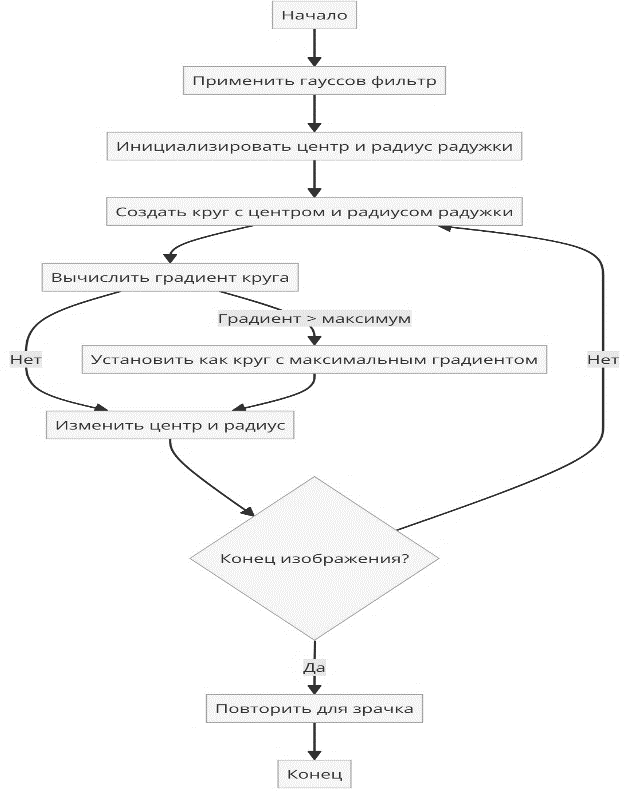
\includegraphics[width=0.6\textwidth]{assets/83}
	\caption*{Рис. 1 - Блок-схема алгоритма Даугмана}
\end{figure}

\begin{multicols}{2}
\emph{Набор данных.} В рамках данной работы эксперимент был проведен с
использованием четырех различных баз данных изображений, среди которых
три базы данных лиц и одна база данных изображений глаз. Конкретно
использовались следующие базы данных: ORL Face Database, YALE Face
Database, Real Face Database и CASIA-IrisV1 Database.

База данных ORL Face является одной из наиболее часто используемых в
исследованиях по распознаванию лиц. Она включает 600 изображений 60
различных людей, по 10 изображений на каждого человека. Вариации
выражений лица включают открытые/закрытые глаза, улыбку/отсутствие
улыбки, а также наличие или отсутствие очков.

База данных YALE Face является широко используемым набором изображений в
оттенках серого и содержит 265 изображений 25 различных людей в формате
GIF. У каждого человека имеется по 21 изображений, представляющих
различные выражения лица: центральное освещение, счастливое, левое
освещение, без очков, нормальное, правое освещение, удивленное,
грустное, сонное и подмигивающее.

Также использовалась база данных реальных лиц.

База данных CASIA-IrisV1 содержит изображения глаз.

Особенностью данной работы является использование набора данных реальных
лиц для эксперимента. Этот набор данных включает 500 изображений 70
различных людей, по 6 изображений каждого человека. В наборе данных
представлены как мужчины, так и женщины разного возраста. Изображения
обладают разнообразием выражений и особенностей, таких как закрытые и
открытые глаза, наличие солнцезащитных очков, хиджаба, бороды и усов.
\end{multicols}

\begin{figure}[H]
	\centering
	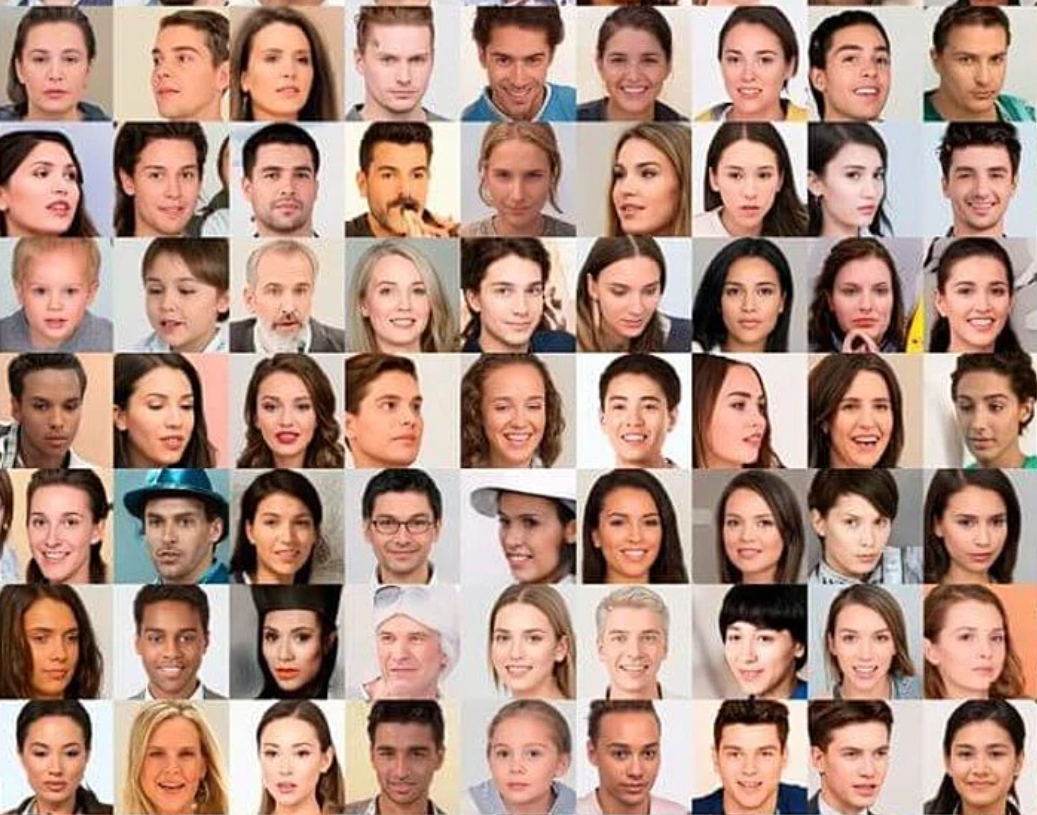
\includegraphics[width=0.8\textwidth]{assets/84}
	\caption*{Рис. 2 - Набор данных о реальном лице}
\end{figure}

\begin{figure}[H]
	\centering
	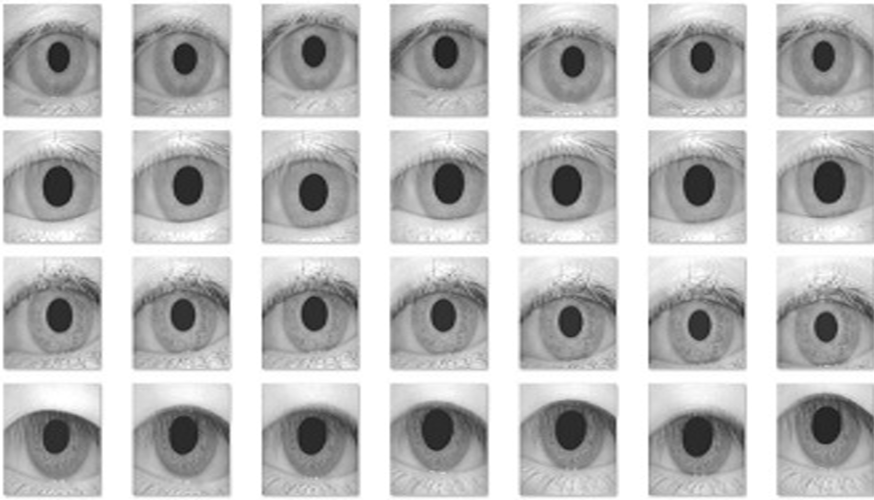
\includegraphics[width=0.8\textwidth]{assets/85}
	\caption*{Рис.3 - База данных изображений радужной оболочки КАССИИ версии 1.0}
\end{figure}

\begin{multicols}{2}
База данных изображений радужной оболочки CASIA версии 1.0
(CASIA-IrisV1) является широко известной и включает 756 изображений
радужной оболочки 108 глаз {[}20{]}. Для каждого глаза было получено по
семь изображений с использованием камеры CASIA close-up iris camera в
ходе двух разных сеансов. В первом сеансе было получено три изображения,
а во втором --- четыре. Все изображения представлены в формате BMP с
разрешением 320x280 пикселей. Эти три различных набора данных,
использованные в данной работе, позволяют сравнить эффективность
предложенного метода с эффективностью традиционного алгоритма PCA.

Для реализации комбинированного алгоритма RSA и алгоритма Даугмана
использовалась библиотека OpenCV. Это популярная библиотека с открытым
исходным кодом для компьютерного зрения и машинного обучения. В рамках
данного исследования эта платформа также применялась для обучения и
тестирования изображений лиц и радужной оболочки глаза.

\emph{{\bfseries Метод.}} Рабочая процедура комбинированного метода
PCA-Daugman включает распознавание лиц и радужной оболочки глаза. Эти
этапы включают множество операций, таких как получение, обработка,
извлечение признаков, сопоставление, нормализация и комбинирование
данных.

Процесс работы комбинированного метода PCA-Daugman пошагово представлен
на блок-схеме (рис. 4).

Распознавание лиц: для распознавания лиц используется метод анализа
главных компонент (PCA), который извлекает признаки, называемые
"собственными чертами лица", из изображений лиц. Анализ главных
компонент применяется к базам данных изображений ORL, YALE и Real Face
Database. В этом модуле выполняются следующие шаги:

- на этом этапе загружаются изображения лиц из базы данных.

- на этапе предварительной обработки выполняются операции, такие как
масштабирование, регулировка контрастности и яркости, чтобы изображения
лиц соответствовали требованиям базы данных. Нормализация гистограммы
является широко известным методом предварительной обработки изображений
лиц.

- для извлечения признаков используется метод анализа главных компонент,
который создает набор собственных поверхностей. Этапы извлечения
признаков включают:

- вычисление векторов изображений и нахождение среднего вектора для всех
изображений.
\end{multicols}

\begin{figure}[H]
	\centering
	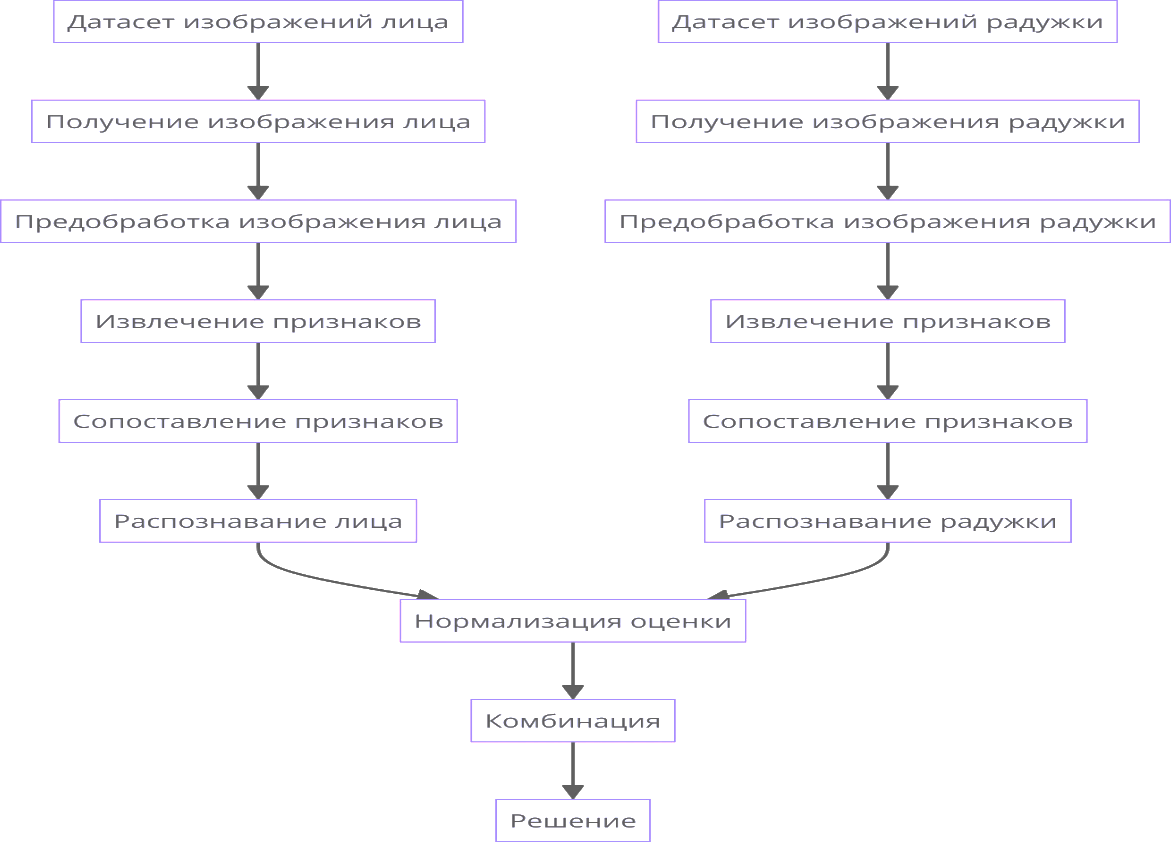
\includegraphics[width=0.6\textwidth]{assets/86}
	\caption*{Рис. 4 - Блок-схема распознавания лица и радужной оболочки глаза с использованием комбинированного PCA-Daugman}
\end{figure}

\begin{multicols}{2}
Извлечение вектора среднего изображения из вектора трехмерного
изображения осуществляется путем вычитания вектора среднего изображения
из вектора трехмерного изображения. Вычисление ковариационной матрицы
позволяет определить собственные значения и собственные векторы.
Собственные значения вычисляются с использованием ковариационной и
единичной матриц, а собственные векторы --- на основе полученных
собственных значений. Набор собственных поверхностей создается с
использованием собственных значений и собственных векторов. Вектор
признаков для всех изображений из обучающего набора определяется
посредством вычисления веса/вектора признаков. Тестовое изображение
выбирается из набора тестовых изображений.

Соответствие признакам рассчитывается на основе евклидова расстояния
между обучающими и тестовыми векторами признаков. Результаты каждого
теста сохраняются для использования в комбинированном методе
распознавания лица и радужной оболочки глаза PCA-Даугмана. Метод
распознавания радужной оболочки глаза Даугмана используется для
сегментации изображений глаз и применяется к базе данных изображений
глаз CASIA. Для распознавания радужной оболочки глаза загружаются
изображения радужной оболочки из базы данных CASIA, выполняется
предварительная обработка изображений с использованием функций
локализации и нормализации радужной оболочки, кодируются признаки
нормализованного рисунка радужной оболочки глаза для обучающего и
тестового набора изображений с использованием одномерных вейвлетов
Логарифма-Габора, сохраняются закодированные признаки в виде шаблонов и
масок, и рассчитывается оценка соответствия с использованием расстояния
Хэмминга между шаблонами и масками для обучающих и тестовых изображений.
Соответствующие результаты каждого теста сохраняются для использования в
комбинированном методе распознавания лиц и радужной оболочки глаза
PCA-Даугмана. При использовании комбинированного метода PCA-Даугмана
распознавание лица и радужной оболочки глаза выполняются совместно, что
является основной целью данного исследования. На этом этапе используются
оценки, полученные на этапах распознавания лица и радужной оболочки
глаза. Для распознавания лиц применяется метод PCA для выделения
признаков, а для расчета оценки соответствия используется евклидово
расстояние. В распознавании радужной оболочки глаза метод Даугмана
используется для выделения признаков, а для определения оценки
соответствия используется расстояние Хэмминга. Оба соответствующих балла
нормализуются с использованием метода min-max нормализации с общей
областью и диапазоном. В данной работе используется правило взвешенной
суммы для метода комбинирования уровней баллов. Окончательное решение об
идентификации человека принимается на основе совокупных показателей
распознавания лица и радужной оболочки глаза.

{\bfseries Результаты и обсуждение.} При использовании комбинированной
методики PCA-Daugman точность мультимодальной системы распознавания лиц
и радужной оболочки глаза для различных сценариев различна, но явно
превосходит точность унимодального распознавания, использующего PCA или
алгоритм Даугмана по отдельности. Точность рассчитывается с точностью до
50 эпох для случайных тестовых изображений.

\emph{Результаты.} Показатели распознавания для базы данных Borland C
ASIA приведены на рисунке 5.

Производительность распознавания лиц для базы данных ORACLE,
распознавания радужной оболочки глаза для базы данных CATIA, а также
обеих баз данных для комбинированного распознавания лиц и радужной
оболочки глаза оценивается на основе случайно выбранных тестовых
изображений. Из рисунка 5 следует, что точность распознавания лиц и
радужной оболочки глаза с применением комбинированного метода
PCA-Daugman значительно превосходит унимодальные методы для баз данных
ORL и CASIA. Производительность для набора данных Yale была также
оценена с использованием методов PCA, Daugman и их комбинированного
подхода. Результаты распознавания для баз данных Yale и CASIA
представлены на рисунке 6.
\end{multicols}

\begin{figure}[H]
    \centering
    \begin{subfigure}[b]{0.45\textwidth}
        \centering
        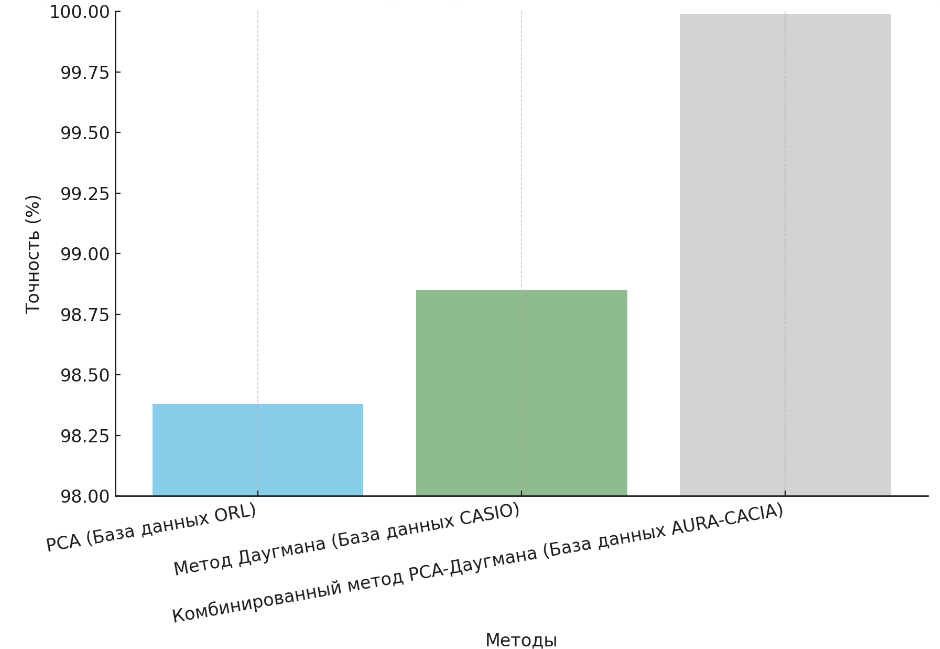
\includegraphics[width=\textwidth]{assets/87}
		\caption*{Рис. 5 - Производительность распознавания лиц и радужной оболочки глаза для базы данных Borland C ASIA}
    \end{subfigure}
    \hfill
    \begin{subfigure}[b]{0.45\textwidth}
        \centering
        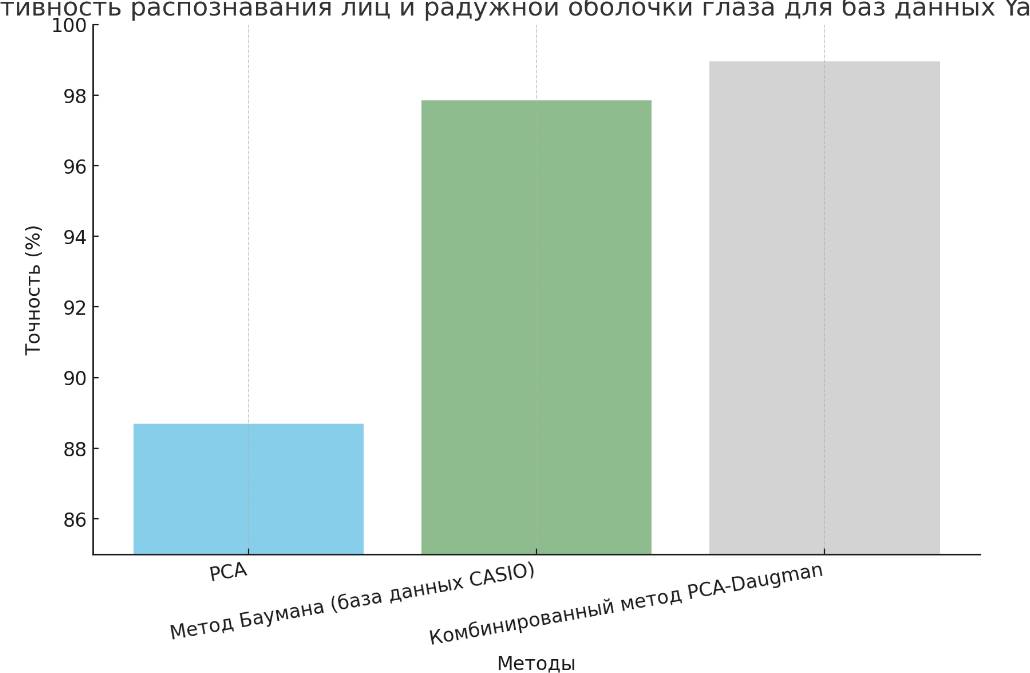
\includegraphics[width=\textwidth]{assets/88}
		\caption*{Рис. 6 - Эффективность распознавания лиц и радужной оболочки глаза для баз данных Yale и CASIO}
    \end{subfigure}
\end{figure}

\begin{figure}[H]
	\centering
	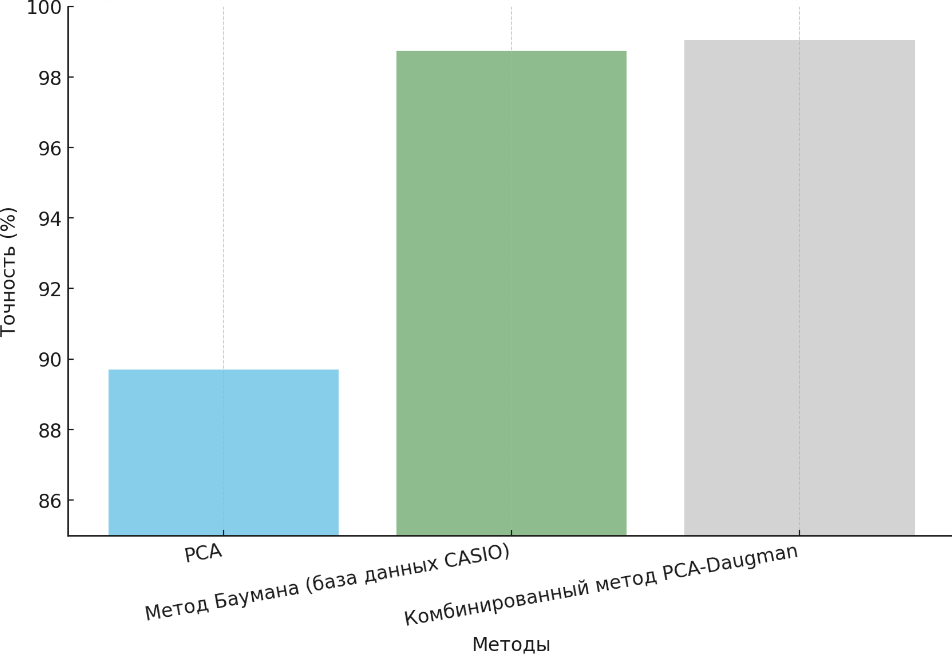
\includegraphics[width=0.45\textwidth]{assets/89}
	\caption*{Рис. 7 - Эффективность распознавания лиц и радужной оболочки глаза для баз данных Yale и CASIO}
\end{figure}

\begin{multicols}{2}
Из рисунока 6 следует, что производительность комбинированного метода
PCA и алгоритма Даугмана для баз данных Yale и CASIA превосходит
результаты, достигнутые с использованием одномодальных методов PCA и
алгоритма Даугмана. База данных Real Face включает реальные изображения,
используемые для оценки эффективности данного подхода. Эффективность
распознавания с применением методов PCA, Daugman и их комбинированного
подхода для базы данных Real Face и базы данных CASIA представлена на
рисунке 7.

Из рисунока 7 следует, что точность распознавания с использованием
алгоритма PCA и метода Даугмана для базы данных Real Face и CASIA
значительно ниже, чем при применении комбинированного метода PCA и
Даугмана.

\emph{Обсуждение.} Из анализа результатов становится очевидно, что
эффективность распознавания лиц с использованием комбинированного метода
PCA-Daugman превосходит результаты, полученные при использовании методов
PCA и Daugman по отдельности. Эксперименты с комбинированным методом
PCA-Daugman были проведены на четырех различных базах данных
изображений: ORL, Yale, Real Face и CASIA. Точность данного метода
значительно выше по сравнению с распознаванием лиц и радужной оболочки
глаза по отдельности для идентификации человека. Результаты
демонстрируют, что данный исследовательский метод показывает высокую
эффективность. Таким образом, комбинированный метод PCA-Daugman доказал
свою эффективность для мультимодального распознавания лица и радужной
оболочки глаза.

{\bfseries Выводы.} Целью данного исследования являлась разработка
комбинированного метода PCA-Daugman, который обеспечивает улучшенные
результаты мультимодального распознавания лиц и радужной оболочки глаза.
Предложенный метод предоставляет решение для более эффективной
идентификации человека, используя особенности лица и радужной оболочки
глаза. Он способен идентифицировать людей с длинной бородой и усами, а
также тех, кто носит солнцезащитные очки или шарф. В дальнейшем
планируется использование более расширенных и реалистичных баз данных
сложных изображений, а также применение более динамичных и эффективных
алгоритмов для повышения точности и уменьшения сложности процесса. Также
предполагается внедрение передовых возможностей искусственного
интеллекта для повышения адаптивности и надежности системы распознавания
в ближайшем.
\end{multicols}

\begin{center}
{\bfseries Литература}
\end{center}

\begin{noparindent}
1.Boyd, A., Fang, Z., Czajka, A., \& Bowyer, K. W. Iris presentation
attack detection: Where are we now?//Pattern Recognition
Letters.-2020.-Vol.138.-P.483-489.

DOI 10.1016/j.patrec.2020.08.018

2.Kaur P. et al. Facial-recognition algorithms: A literature review
//Medicine, Science and the Law. -2020. - Vol.60(2).- P. 131-139. DOI
10.1177/0025802419893168

3.Min W. Y., Romanova E., Lisovec Y., San,A. M. Application of
statistical data processing for solving the problem of face recognition
by using principal components analysis method // 2019 IEEE Conference of
Russian Young Researchers in Electrical and Electronic Engineering
(EIConRus), Saint Petersburg and Moscow, Russia.-2019.-P.2208-2212.

DOI 10.1109/EIConRus.2019.8657240

4.AlFawwaz B. M. et al. Multi-Resolution Discrete Cosine Transform
Fusion Technique Face Recognition Model //Data.- 2022. -Vol. 7(6). - P.
80. DOI 10.3390/data7060080

5.Trokielewicz M., Czajka A., Maciejewicz P. Post-mortem iris
recognition with deep-learning-based image segmentation //Image and
Vision Computing. -2020. - Vol. 94 94:103866

DOI 10.1016/j.imavis.2019.103866

6.Farouk R. H., Mohsen H., El-Latif Y. M. A. A proposed biometric
technique for improving iris recognition //International Journal of
Computational Intelligence Systems. -2022. - Vol. 15.-№. 1. DOI
10.1007/s44196-022-00135-z

7.Alam M. M. et al. Combined PCA-Daugman method: An Efficient technique
for face and iris recognition //Journal of Advances in Mathematics and
Computer Science. - 2020.-Vol. 23.- P. 34-44. DOI

10.9734/jamcs/2020/v35i530280

8.Soviany S., Soviany C. Data Fusion in Multimodal Biometry
//Breakthroughs in Digital Biometrics and

Forensics.//Cham: Springer
International Publishing, 2022.-P.49-88.

DOI 10.1007/978-3-031-10706-1\_3

9.Priya A. S., Mukesh R. GA based Feature Selection for Multimodal
Biometric Authentication // Indian Journal of Computer Science and
Engineering. -2021. -Vol.12(2).-P.526-538.

DOI:10.21817/indjcse/2021/v12i2/211202163

10.Jadhav S. B., Deshmukh N. K., Humbe V. T. HDL-PI: hybrid DeepLearning
technique for person identification using multimodal finger print, iris
and face biometric features //Multimedia Tools and Applications. - 2023.
-Vol. 82(19). -P. 30039-30064.

11.Nguyen, K., Proença, H., Alonso-Fernandez, F. Deep Learning for Iris
Recognition: A Survey. -- 2022. DOI 10.48550/arXiv.2210.05866

12.Swapna, M., Sharma, Y. K., Prasad, B. A survey on face recognition
using convolutional neural network // Data Engineering and Communication
Technology: Proceedings of 3rd ICDECT-2K19, Springer. -2020. - P.
649-661. DOI:10.1007/978-981-15-1097-7\_54

13.Minaee, S., Abdolrashidi, A. Deepiris: Iris recognition using a deep
learning approach. -2019. DOI

10.48550/arXiv.1907.09380

14.Alaslni, M. G., Elrefaei, L. A. Transfer learning with convolutional
neural networks for iris recognition // Int. J. Artif. Intell. Appl. -
2019. --Vol. 10(5). --P. 49-66. DOI 10.5121/ijaia.2019.10505

15.Ebrahimpour, N., Ayden, M. A., Altay, B. Liveness control in face
recognition with deep learning methods // The European Journal of
Research and Development. - 2022. -Vol. 2(2).-P. 92-101.

DOI 10.56038/ejrnd.v2i2.36

16.Kunda, D., Chishimba, M. A survey of android mobile phone
authentication schemes // Mobile Networks and Applications.- 2021.-Vol.
26(6). -P. 2558-2566. DOI 10.1007/s11036-018-1099-7

17.Marcel S., Fierrez J., Evans N. (ed.). Handbook of Biometric
Anti-Spoofing: Presentation Attack Detection and Vulnerability
Assessment.Berlin, Germany: Springer, 2023.-564 p.

ISBN-109811952876

18.Minaee S. et al. Biometrics recognition using deep learning: A survey
//Artificial Intelligence Review. -2023. -Vol. 56(8.) - P. 8647-8695.

19.Dargan S., Kumar M. A comprehensive survey on the biometric
recognition systems based on physiological and behavioral modalities
//Expert Systems with Applications. -2020. -Vol. 143.

DOI 10.1016/j.eswa.2019.113114

20.Biometrics ideal test.
--URL:http://biometrics.idealtest.org/dbDetailForUser.do?id=1 (дата обращения:

19.06.2024)
\end{noparindent}

\emph{{\bfseries Сведения об авторах}}

\begin{noparindent}
Мусайф М. -- докторант Евразийского национального университета им. Л. Н.
Гумилева, Астана, Казахстан, e-mail: kzldkz@gmail.com;

Кинтаново А. - и.о. доцента кафедры технологий искусственного интеллекта
Евразийского национального университета им. Л.Н. Гумилева, Астана,
е-mail:Kintonova\_AZh@enu.kz;

Назырова А. - старший преподаватель Международного университета Астаны,
Астана, Казахстан,

е-mail: ayzhan.nazyrova@gmail.com;

Алтынбек С.- доктор PhD, Казахский университет технологии и бизнеса им.
К.Кулажанова,Астана, Казахстан, е-mail: serik\_aa@bk.ru;

Калдарова М. - старший преподаватель Международного университета Астаны,
Астана, Казахстан,

е-mail: kmiraj82@mail.ru.
\end{noparindent}

\emph{{\bfseries Information about the authors}}

\begin{noparindent}
Mussaif M.-- doctorial student of the L. N. Gumilev Eurasian National
University, Astana, Kazakhstan,

е-mail: kzldkz@gmail.com;

Kintanovo A. - Acting Associate Professor of the Department of
Artificial Intelligence Technology of the L.N. Gumilyov Eurasian
National University, Astana, е-mail:Kintonova\_AZh@enu.kz;

NazyrovaA. - senior lecturer of the Astana International University,
Astana, Kazakhstan,

е-mail: ayzhan.nazyrova@gmail.com;

Altynbek S. - doktorPhD, K. Kulazhanov Kazakh University of Technology
and Business, Astana, Kazakhstan,

е-mail: serik\_aa@bk.ru;

Kaldarova M. - senior lecturer at Astana International University,
Astana, Kazakhstan, е-mail: kmiraj82@mail.ru.
\end{noparindent}
